% Options for packages loaded elsewhere
\PassOptionsToPackage{unicode}{hyperref}
\PassOptionsToPackage{hyphens}{url}
%
\documentclass[
]{article}
\usepackage{amsmath,amssymb}
\usepackage{lmodern}
\usepackage{iftex}
\ifPDFTeX
  \usepackage[T1]{fontenc}
  \usepackage[utf8]{inputenc}
  \usepackage{textcomp} % provide euro and other symbols
\else % if luatex or xetex
  \usepackage{unicode-math}
  \defaultfontfeatures{Scale=MatchLowercase}
  \defaultfontfeatures[\rmfamily]{Ligatures=TeX,Scale=1}
\fi
% Use upquote if available, for straight quotes in verbatim environments
\IfFileExists{upquote.sty}{\usepackage{upquote}}{}
\IfFileExists{microtype.sty}{% use microtype if available
  \usepackage[]{microtype}
  \UseMicrotypeSet[protrusion]{basicmath} % disable protrusion for tt fonts
}{}
\makeatletter
\@ifundefined{KOMAClassName}{% if non-KOMA class
  \IfFileExists{parskip.sty}{%
    \usepackage{parskip}
  }{% else
    \setlength{\parindent}{0pt}
    \setlength{\parskip}{6pt plus 2pt minus 1pt}}
}{% if KOMA class
  \KOMAoptions{parskip=half}}
\makeatother
\usepackage{xcolor}
\IfFileExists{xurl.sty}{\usepackage{xurl}}{} % add URL line breaks if available
\IfFileExists{bookmark.sty}{\usepackage{bookmark}}{\usepackage{hyperref}}
\hypersetup{
  pdftitle={Relatório trabalho prático 1},
  pdfauthor={César A. Galvão 19/0011572; Gabriela Carneiro 18/0120816},
  hidelinks,
  pdfcreator={LaTeX via pandoc}}
\urlstyle{same} % disable monospaced font for URLs
\usepackage[margin=1in]{geometry}
\usepackage{color}
\usepackage{fancyvrb}
\newcommand{\VerbBar}{|}
\newcommand{\VERB}{\Verb[commandchars=\\\{\}]}
\DefineVerbatimEnvironment{Highlighting}{Verbatim}{commandchars=\\\{\}}
% Add ',fontsize=\small' for more characters per line
\usepackage{framed}
\definecolor{shadecolor}{RGB}{248,248,248}
\newenvironment{Shaded}{\begin{snugshade}}{\end{snugshade}}
\newcommand{\AlertTok}[1]{\textcolor[rgb]{0.94,0.16,0.16}{#1}}
\newcommand{\AnnotationTok}[1]{\textcolor[rgb]{0.56,0.35,0.01}{\textbf{\textit{#1}}}}
\newcommand{\AttributeTok}[1]{\textcolor[rgb]{0.77,0.63,0.00}{#1}}
\newcommand{\BaseNTok}[1]{\textcolor[rgb]{0.00,0.00,0.81}{#1}}
\newcommand{\BuiltInTok}[1]{#1}
\newcommand{\CharTok}[1]{\textcolor[rgb]{0.31,0.60,0.02}{#1}}
\newcommand{\CommentTok}[1]{\textcolor[rgb]{0.56,0.35,0.01}{\textit{#1}}}
\newcommand{\CommentVarTok}[1]{\textcolor[rgb]{0.56,0.35,0.01}{\textbf{\textit{#1}}}}
\newcommand{\ConstantTok}[1]{\textcolor[rgb]{0.00,0.00,0.00}{#1}}
\newcommand{\ControlFlowTok}[1]{\textcolor[rgb]{0.13,0.29,0.53}{\textbf{#1}}}
\newcommand{\DataTypeTok}[1]{\textcolor[rgb]{0.13,0.29,0.53}{#1}}
\newcommand{\DecValTok}[1]{\textcolor[rgb]{0.00,0.00,0.81}{#1}}
\newcommand{\DocumentationTok}[1]{\textcolor[rgb]{0.56,0.35,0.01}{\textbf{\textit{#1}}}}
\newcommand{\ErrorTok}[1]{\textcolor[rgb]{0.64,0.00,0.00}{\textbf{#1}}}
\newcommand{\ExtensionTok}[1]{#1}
\newcommand{\FloatTok}[1]{\textcolor[rgb]{0.00,0.00,0.81}{#1}}
\newcommand{\FunctionTok}[1]{\textcolor[rgb]{0.00,0.00,0.00}{#1}}
\newcommand{\ImportTok}[1]{#1}
\newcommand{\InformationTok}[1]{\textcolor[rgb]{0.56,0.35,0.01}{\textbf{\textit{#1}}}}
\newcommand{\KeywordTok}[1]{\textcolor[rgb]{0.13,0.29,0.53}{\textbf{#1}}}
\newcommand{\NormalTok}[1]{#1}
\newcommand{\OperatorTok}[1]{\textcolor[rgb]{0.81,0.36,0.00}{\textbf{#1}}}
\newcommand{\OtherTok}[1]{\textcolor[rgb]{0.56,0.35,0.01}{#1}}
\newcommand{\PreprocessorTok}[1]{\textcolor[rgb]{0.56,0.35,0.01}{\textit{#1}}}
\newcommand{\RegionMarkerTok}[1]{#1}
\newcommand{\SpecialCharTok}[1]{\textcolor[rgb]{0.00,0.00,0.00}{#1}}
\newcommand{\SpecialStringTok}[1]{\textcolor[rgb]{0.31,0.60,0.02}{#1}}
\newcommand{\StringTok}[1]{\textcolor[rgb]{0.31,0.60,0.02}{#1}}
\newcommand{\VariableTok}[1]{\textcolor[rgb]{0.00,0.00,0.00}{#1}}
\newcommand{\VerbatimStringTok}[1]{\textcolor[rgb]{0.31,0.60,0.02}{#1}}
\newcommand{\WarningTok}[1]{\textcolor[rgb]{0.56,0.35,0.01}{\textbf{\textit{#1}}}}
\usepackage{graphicx}
\makeatletter
\def\maxwidth{\ifdim\Gin@nat@width>\linewidth\linewidth\else\Gin@nat@width\fi}
\def\maxheight{\ifdim\Gin@nat@height>\textheight\textheight\else\Gin@nat@height\fi}
\makeatother
% Scale images if necessary, so that they will not overflow the page
% margins by default, and it is still possible to overwrite the defaults
% using explicit options in \includegraphics[width, height, ...]{}
\setkeys{Gin}{width=\maxwidth,height=\maxheight,keepaspectratio}
% Set default figure placement to htbp
\makeatletter
\def\fps@figure{htbp}
\makeatother
\setlength{\emergencystretch}{3em} % prevent overfull lines
\providecommand{\tightlist}{%
  \setlength{\itemsep}{0pt}\setlength{\parskip}{0pt}}
\setcounter{secnumdepth}{5}
\usepackage{helvet} \renewcommand\familydefault{\sfdefault}
\usepackage{booktabs}
\usepackage{longtable}
\usepackage{array}
\usepackage{multirow}
\usepackage{wrapfig}
\usepackage{float}
\usepackage{colortbl}
\usepackage{pdflscape}
\usepackage{tabu}
\usepackage{threeparttable}
\usepackage{threeparttablex}
\usepackage[normalem]{ulem}
\usepackage{makecell}
\usepackage{xcolor}
\ifLuaTeX
  \usepackage{selnolig}  % disable illegal ligatures
\fi

\title{Relatório trabalho prático 1}
\author{César A. Galvão 19/0011572 \and Gabriela Carneiro 18/0120816}
\date{26 de June de 2022}

\begin{document}
\maketitle

\newpage{}

{
\setcounter{tocdepth}{2}
\tableofcontents
}
\let\oldsection\section
\renewcommand\section{\clearpage\oldsection}

\begin{center} 

\textbf{Resumo} 

\end{center}

Nesta atividade foram implementadas em R três métodos de ordenação --
seleção, inserção e QuickSort -- e seus desempenhos foram medidos por
meio de tempo de execução, número de comparações entre elementos do
vetor e número de movimentações dos elementos do vetor. Os três métodos
foram testados com tamanhos variados de amostras, variando o tamanho de
500 a 50.000, assim como vetores previamente organizados de quatro
formas: ordenados, ordenados de maneira inversa, parcialmente
aleatorizados (cerca de 10\% dos elementos têm posições aleatórias) e
completamente aleatorizados. As duas últimas formas foram executadas 100
vezes e as medidas de interesse são representadas por suas médias.
Enquanto (INSERIR AQUI OBSERVAÇÃO), observou-se que (INSERIR OUTRA
OBSERVAÇÃO). Conclui-se que (INSERIR CONCLUSAO).\footnote{Todos os
  documentos desse relatório podem ser verificados no repositório
  \url{https://github.com/cesar-galvao/Estatistica-computacional}}

\hypertarget{introduuxe7uxe3o}{%
\section{Introdução}\label{introduuxe7uxe3o}}

\hypertarget{muxe9todos-de-ordenauxe7uxe3o}{%
\subsection{Métodos de ordenação}\label{muxe9todos-de-ordenauxe7uxe3o}}

O ordenamento de dados tem papel crucial no campo das ciências da
computação. Os vários tipos de algoritmos de ordenação diferem entre si
em termos de eficiência, uso de memória, complexidade, dentre outros
fatores. Por esse motivo, esses algoritmos tem sito extensamente
analisados por meio de pesquisas. Nesse contexto, cada algoritmo
desenvolvido para ordenamento de dados tem seus benefícios e limitações,
sendo que o desempenho deles pode ser otimizado de diversas maneiras
(Zutshi \& Goswami, 2021)\footnote{\href{https://www.sciencedirect.com/science/article/pii/S2667096821000355}{Zutshi,
  A, Goswami, D. (2021) \emph{Systematic review and exploration of new
  avenues for sorting algorithm}}}.

Na ciência da computação, a eficiência entre algoritmos é comparada
geralmente em termos do tempo de execução. Muitos dos algoritmos de
ordenação têm complexidade linear ou quadrática. Destes muitos tem
complexidade quadrática \(O(n^2)\) como pior caso e complexidade linear
como melhor caso, sendo que o desempenho dos algoritmos \(O(n^2)\) tende
a cair conforme a quantidade de dados aumenta. Ainda, alguns algoritmos
tem a complexidade \(O(n \log n)\) tanto no pior caso quanto em seu
melhor caso (Zutshi \& Goswami, 2021).

\hypertarget{ordenauxe7uxe3o-por-seleuxe7uxe3o}{%
\subsubsection{Ordenação por
seleção}\label{ordenauxe7uxe3o-por-seleuxe7uxe3o}}

O método de ordenação por seleção percorre a sequencia de dados e
``seleciona'' cada elemento que não está em sua posição correta. Em
seguida, ele o troca de lugar com o elemento que está na primeira
posição. O algoritmo executa esse mesmo procedimento para o restante da
lista de dados.

Estas operações quando executadas têm complexidade quadrática, sendo que
a busca pelo menor elemento da operação custa \(n - 1\) passos na
primeira iteração. Em seguida a operação custa \(n - 2\) na segunda
operação e assim por diante. Dessa forma, o custo total é dado pela soma
da progressão aritmética \(\sum\limits_{i = 1}^{n-1} a_i\) de razão
\(r = 1\), com \(a_1 = 1\) e \(a_{n-1} = (n-1)\). Dessa forma, o tempo
de execução do algoritmo é:

\begin{equation}
  \frac{n(1+(n-1))}{2} = \frac{n^2}{2}
\end{equation}

\hypertarget{ordenauxe7uxe3o-por-inseruxe7uxe3o}{%
\subsubsection{Ordenação por
inserção}\label{ordenauxe7uxe3o-por-inseruxe7uxe3o}}

Esse tipo de método de ordenação ``insere'' cada elemento desordenado
dos dados em sua posição correta. Ou seja, esse tipo de ordenação tem
como rotina base a inserção ordenada, que basicamente compara o elemento
que está sendo ordenado com os elementos anteriores a ele e só efetua
uma movimentação quando tal elemento é maior que elemento imediatamente
e sua esquerda ou quando ele ocupa a primeira posição da sequência. As
operaçãoes, assim como o método do ordenação por seleção, são de ordem
quadrática, em seu pior caso. Em seu melhor caso, quando os elementos já
estão ordenados, o custo total é de \(O(n)\).

Assim como no caso de ordenação mencionado anteriomente, o custo total é
dado pela soma da progressão aritmética
\(\sum\limits_{i = 1}^{n-1} a_i\) de razão \(r = 1\), com \(a_1 = 1\) e
\(a_{n-1} = (n-1)\). Dessa forma, o tempo de execução do algoritmo é:

\begin{equation}
  \frac{n(1+(n-1))}{2} = \frac{n^2}{2}
\end{equation}

\hypertarget{quick-sort}{%
\subsubsection{Quick Sort}\label{quick-sort}}

O Quicksort geralmente é implementado recursivamente. Um pivô aleatório
é escolhido e todos os elementos são reorganizados em torno do pivô em
ordem crescente mantendo-o como referência. A escolha do pivô determina
a complexidade do quicksort sendo que em algumas versões, nos melhores
casos, o algoritmo tem complexidade de \(O(n \log n)\). No entanto, se o
pivô for selecionado em uma das extremidades da sequencia, ele passa a
ter complexidade de \(O(n^2)\).

Escolher um pivô aleatorimente é um boa estratégia para diminuir
significativamente a probabilidade de ocorrência do pior caso, já que,
para o pior caso acontecer, o pivô escolhido deveria ser sempre o pior
tendo uma probabilidade de ocorrência

\begin{equation}
  p = \frac{1}{n!}.
\end{equation}

\hypertarget{sec144}{%
\subsubsection{Comparação entre métodos de ordenação}\label{sec144}}

Comparando os diferentes tipos de estratégia de ordenação, é esperado
que o método de ordenação por seleção efetue menos trocas do que o
método de ordenação por inserção, pois há uma troca apenas por iteração.
Desse modo, o algoritmo efetua \(n\) trocas. Já o método de inserção
efetua ao menos uma troca por iteração.

Contudo, este efetua menos comparações do que o algoritmo de seleção,
pois nem sempre o elemento a ser inserido de forma ordenada deve ir até
o final do vetor. Isso só ocorre no pior caso, isto é, quando os
elementos estão ordenado em ordem decrescente. O algoritmo de seleção
precisa comparar todos os elementos restantes a cada iteração para
determinar qual é o menor deles.

Ambos os métodos citados acima estão na mesma classe de complexidade
(\(O(n^2)\)). No entanto, o método de inserção apresenta melhor
desempenho do que o método de seleção na prática.

Entre os três métodos, o Quick Sort é o mais eficiente. Tendo uma
complexidade de \(O(n \log n)\), exceto no seu pior cenário, o método
atinge a mesma complexidade dos outros dois tipos avaliados.

\hypertarget{muxe9todo}{%
\section{Método}\label{muxe9todo}}

\hypertarget{testes-de-desempenho}{%
\subsection{Testes de desempenho}\label{testes-de-desempenho}}

Os testes de desempenho realizados para cada um dos algoritmos de
ordenação tomaram em conta duas dimensões: tamanho de amostra e
ordenação prévia do vetor a ser ordenado.

Para poder comparar os métodos, três medidas foram feitas para todos os
tamanhos de amostra: contagem da quantidade de movimentações, quantidade
de comparações entre elementos e tempo de execução. Vetores ordenados
nas duas direções tiveram testes realizados apenas uma vez, enquanto
aqueles que possuíam algum elemento aleatório foram realizados cem vezes
e os valores considerados para comparação são as médias dessas crm
realizações de teste.

\hypertarget{amostragem}{%
\subsection{Amostragem}\label{amostragem}}

As amostras foram criadas utilizando a função
\texttt{gera.amostra(size,\ ordem,\ seed)} disponível no código anexo.
Os argumentos correspondem a tamanho, ordenamento e seed para a geracao
da aleatoriedade desejada. A função retorna uma lista de dois elementos:
o vetor e o método de ordenação desejado.

O tamanho da amostra permitido na função é qualquer número inteiro. Não
foram realizados controles para tamanho 0 e números negativos, porém
qualquer número estritamente positivo tem retorno válido. Para os
testes, foram utilizados cinco tamanhos de amostra: 500, 1.000, 5.000,
10.000 e 50.000.

O argumento \emph{ordem} da função recebe uma das quatro ordenações
testadas, quais sejam: completamente ordenado, inversamente ordenado,
completamente aleatorizado e parcialmente aleatorizado. Este caso
compreende 10\% de aleatorizacao dos elementos do vetor.

\hypertarget{implementauxe7uxe3o-do-muxe9todo-de-seleuxe7uxe3o}{%
\subsection{Implementação do método de
seleção}\label{implementauxe7uxe3o-do-muxe9todo-de-seleuxe7uxe3o}}

O método seleção foi implementado na função \texttt{selecao()}, que
recebe a lista da função de amostragem como argumento. Inicialmente, o
elemento \(a_i, i = 1, 2, ..., n-1\), é tomado como mínimo (\(min = i\))
e é comparado aos elementos \(a_j, j = 2, 3, ..., n\) seguintes. Se
\(a_j < a_{min}\), esses elementos são invertidos e o mínimo é
redefinido, \(min = j\). essas operações são realizadas em um laço
\texttt{for} de dois níveis, conforme o código anexo.

\hypertarget{implementauxe7uxe3o-do-muxe9todo-de-inseruxe7uxe3o}{%
\subsection{Implementação do método de
inserção}\label{implementauxe7uxe3o-do-muxe9todo-de-inseruxe7uxe3o}}

O método seleção foi implementado na função \texttt{insercao()}, que
recebe a lista da função de amostragem como argumento. Considerando
\(i = 2, 3, ..., n\) como o iterador primário e \(j = 1, 2, ..., n-1\),
tem-se \(x_i, x_j\) e \(x_{\text{temp}}\). Na primeira iteração,
defini-se \(x_{\text{temp}} = x_i\). Enquanto \(x_j\) e \(j>0\),
redefine-se \(x_{j+1} = x_j\) e \(j = j-1\) até que uma das condições
não sejam mais satisfeitas. Neste momento, reatribui-se
\(x_{j+1} = x_{\text{temp}}\) e itera-se sobre o próximo valor de \(i\).

\hypertarget{implementauxe7uxe3o-do-quicksort}{%
\subsection{Implementação do
Quicksort}\label{implementauxe7uxe3o-do-quicksort}}

Este algoritmo foi implementado em dois níveis: a funcao
\texttt{quick\_base()}, objeto principal de análise, aplica o algoritmo
enquanto \texttt{quick\_completa()} permite o retorno das medidas de
interesse. A ordenação inicia com a seleção de um pivô, aqui selecionado
como a posição mediana do comprimento do vetor, e redistribui os
elementos do vetor. Enquanto os elementos menores que o pivô são
passados para a esquerda dele, os maiores são passados para a direita.
Em seguida, a função recursivamente opera sobre os braços do vetor até
que todo ele esteja ordenado.

\hypertarget{resultados}{%
\section{Resultados}\label{resultados}}

\hypertarget{tempo-de-execuuxe7uxe3o}{%
\subsection{Tempo de execução}\label{tempo-de-execuuxe7uxe3o}}

Na medida em que o número de elementos nas amostras cresce, o tempo de
execução das ordenações também cresce, conforme esperado. Quando as
amostras são geradas com ordenação de elementos em ordem aleatória, é
possível observar que para ordená-la os métodos de ordenação por
inserção e QuickSort levam menos tempo que o método de seleção, fato que
mostra que o metodo de seleção é mais oneroso que os outro dois. O mesmo
pode ser observado quando as amostra está invertida, ordenada ou
parcialmente ordenada.

Porém, de forma inesperada para as amostras de tamando 50.000, o método
de seleção levou mais tempo para ordenar as amostras que já estavam
ordenadas do que as amostras que estavam completamente invertidas. Isso
não é esperado, pois no caso das amostras invertidas tanto o método de
seleção quanto o método se inserção tem seus piores cenários, tendo
desempenho quadrático.

\begin{figure}

{\centering 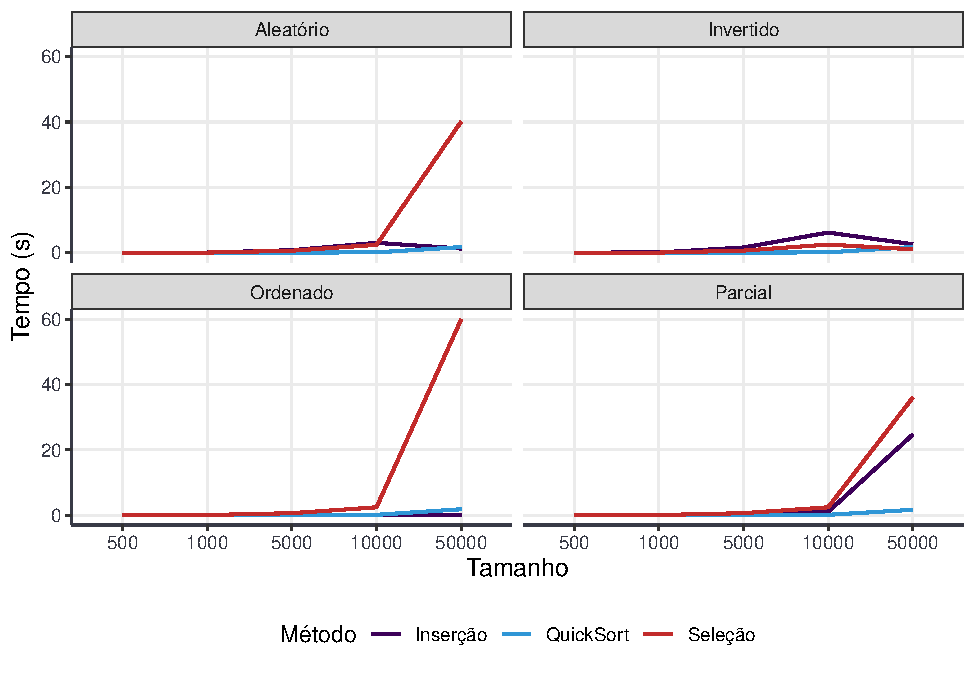
\includegraphics[width=0.75\linewidth]{relatorio_tp1_2_files/figure-latex/grafico-tempo-1} 

}

\caption{Tempo de execução dos métodos desagregado por ordenamento original da amostra}\label{fig:grafico-tempo}
\end{figure}

\hypertarget{nuxfamero-de-comparauxe7uxf5es}{%
\subsection{Número de
comparações}\label{nuxfamero-de-comparauxe7uxf5es}}

Conforme pode ser observado na figura 2, o número de comparações também
tende a crescer conforme o número de elementos das amostras aumenta.
Ainda, para todos os tipos de amostra o método de seleção foi o que fez
o maior número de comparações, principalmente para as amostras maiores
de 10.000 e 50.000 elementos. Esse resultado já é esperado, conforme já
citado no item 1.1.4 da introdução. Cabe apontar que, no caso do
ordenamento Invertido, a linha correspondente ao método de Inserção está
sobreposta àquela do método de Seleção.

\begin{figure}

{\centering 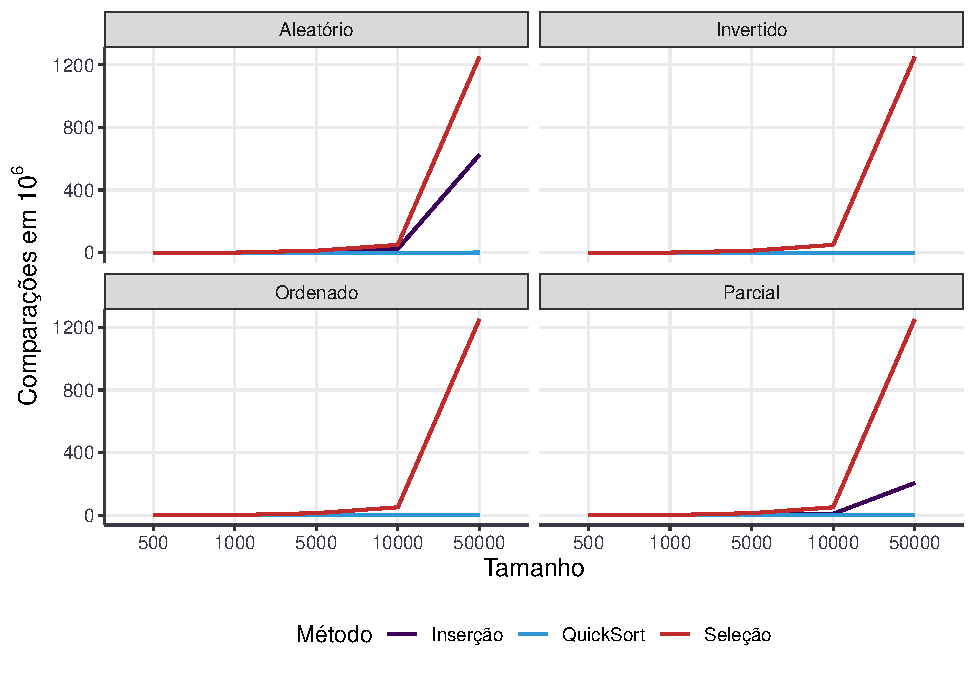
\includegraphics[width=0.75\linewidth]{relatorio_tp1_2_files/figure-latex/grafico-comparacoes-1} 

}

\caption{Quantidade de comparações dos métodos desagregado por ordenamento original da amostra}\label{fig:grafico-comparacoes}
\end{figure}

\break

\hypertarget{nuxfamero-de-movimentauxe7uxf5es}{%
\subsection{Número de
movimentações}\label{nuxfamero-de-movimentauxe7uxf5es}}

De maneira análoga, o número de movimentações também deve crescer a
medida que o número de elementos das amostras cresce. Na figura 3 é
possível observar que o método de ordenação por inserção sempre faz o
maior número de movimentações, conforme já citado anteriormente no item
\protect\hyperlink{sec144}{1.1.4} da introdução, principalmente quando
as amostras estão invertidas, quando esse método tem complexidade
quadrática. Nas amostras ordenadas, não houve movimentações o que já era
esperado. Esse resuldado corrobora que as implementações da contagem das
movimentações foram implementadas de forma correta no desenvolvimentos
das funções dos três métodos de ordenação.

\begin{figure}

{\centering 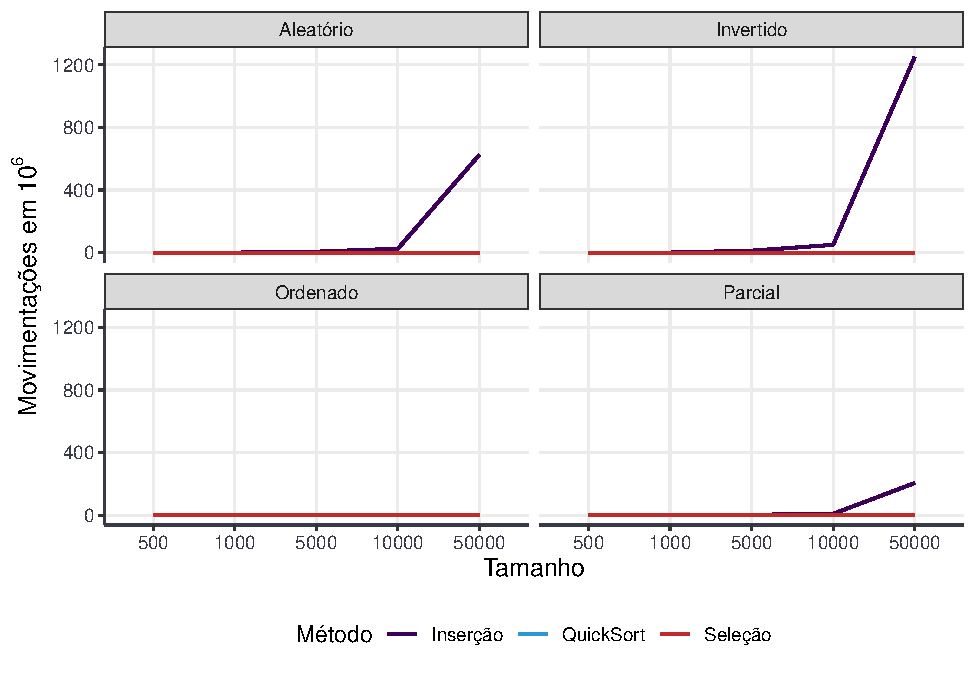
\includegraphics[width=0.75\linewidth]{relatorio_tp1_2_files/figure-latex/grafico-movimentacoes-1} 

}

\caption{Quantidade de movimentações dos métodos desagregado por ordenamento original da amostra}\label{fig:grafico-movimentacoes}
\end{figure}

\hypertarget{conclusao}{%
\section{Conclusao}\label{conclusao}}

Comparar o que se esperava pelas medidas teóricas com o que foi
calculado. Corrobora ou não?

\hypertarget{anexo-a---tabela-com-dados-de-execuuxe7uxe3o-dos-algoritmos}{%
\section*{Anexo A - tabela com dados de execução dos
algoritmos}\label{anexo-a---tabela-com-dados-de-execuuxe7uxe3o-dos-algoritmos}}
\addcontentsline{toc}{section}{Anexo A - tabela com dados de execução
dos algoritmos}

\begin{longtable}[l]{llllll}
\toprule
Método & Tamanho & Ordenamento & Tempo & Comparações & Movimentações\\
\midrule
\endfirsthead
\multicolumn{6}{@{}l}{\textit{(continued)}}\\
\toprule
Método & Tamanho & Ordenamento & Tempo & Comparações & Movimentações\\
\midrule
\endhead

\endfoot
\bottomrule
\endlastfoot
\cellcolor{gray!15}{Inserção} & \cellcolor{gray!15}{500} & \cellcolor{gray!15}{Aleatório} & \cellcolor{gray!15}{0.0073818 secs} & \cellcolor{gray!15}{63175.45} & \cellcolor{gray!15}{63674.45}\\
Inserção & 500 & Invertido & 0.0159225 secs & 125249.00 & 125748.00\\
\cellcolor{gray!15}{Inserção} & \cellcolor{gray!15}{500} & \cellcolor{gray!15}{Ordenado} & \cellcolor{gray!15}{0.0000772 secs} & \cellcolor{gray!15}{499.00} & \cellcolor{gray!15}{998.00}\\
Inserção & 500 & Parcial & 0.0024790 secs & 21346.50 & 21845.50\\
\cellcolor{gray!15}{Inserção} & \cellcolor{gray!15}{1000} & \cellcolor{gray!15}{Aleatório} & \cellcolor{gray!15}{0.0300949 secs} & \cellcolor{gray!15}{251098.85} & \cellcolor{gray!15}{252097.85}\\
Inserção & 1000 & Invertido & 0.0620458 secs & 500499.00 & 501498.00\\
\cellcolor{gray!15}{Inserção} & \cellcolor{gray!15}{1000} & \cellcolor{gray!15}{Ordenado} & \cellcolor{gray!15}{0.0001290 secs} & \cellcolor{gray!15}{999.00} & \cellcolor{gray!15}{1998.00}\\
Inserção & 1000 & Parcial & 0.0100131 secs & 83807.18 & 84806.18\\
\cellcolor{gray!15}{Inserção} & \cellcolor{gray!15}{5000} & \cellcolor{gray!15}{Aleatório} & \cellcolor{gray!15}{0.7530582 secs} & \cellcolor{gray!15}{6247376.11} & \cellcolor{gray!15}{6252375.11}\\
Inserção & 5000 & Invertido & 1.5809329 secs & 12502499.00 & 12507498.00\\
\cellcolor{gray!15}{Inserção} & \cellcolor{gray!15}{5000} & \cellcolor{gray!15}{Ordenado} & \cellcolor{gray!15}{0.0006828 secs} & \cellcolor{gray!15}{4999.00} & \cellcolor{gray!15}{9998.00}\\
Inserção & 5000 & Parcial & 0.2473113 secs & 2052134.50 & 2057133.50\\
\cellcolor{gray!15}{Inserção} & \cellcolor{gray!15}{10000} & \cellcolor{gray!15}{Aleatório} & \cellcolor{gray!15}{3.0103041 secs} & \cellcolor{gray!15}{24992830.95} & \cellcolor{gray!15}{25002829.95}\\
Inserção & 10000 & Invertido & 6.1660368 secs & 50004999.00 & 50014998.00\\
\cellcolor{gray!15}{Inserção} & \cellcolor{gray!15}{10000} & \cellcolor{gray!15}{Ordenado} & \cellcolor{gray!15}{0.0013168 secs} & \cellcolor{gray!15}{9999.00} & \cellcolor{gray!15}{19998.00}\\
Inserção & 10000 & Parcial & 0.9891398 secs & 8209190.67 & 8219189.67\\
\cellcolor{gray!15}{Inserção} & \cellcolor{gray!15}{50000} & \cellcolor{gray!15}{Aleatório} & \cellcolor{gray!15}{1.2550940 secs} & \cellcolor{gray!15}{625139777.91} & \cellcolor{gray!15}{625189776.91}\\
Inserção & 50000 & Invertido & 2.5709911 secs & 1250024999.00 & 1250074998.00\\
\cellcolor{gray!15}{Inserção} & \cellcolor{gray!15}{50000} & \cellcolor{gray!15}{Ordenado} & \cellcolor{gray!15}{0.0066781 secs} & \cellcolor{gray!15}{49999.00} & \cellcolor{gray!15}{99998.00}\\
Inserção & 50000 & Parcial & 24.6829854 secs & 204828410.49 & 204878409.49\\
\cellcolor{gray!15}{QuickSort} & \cellcolor{gray!15}{500} & \cellcolor{gray!15}{Aleatório} & \cellcolor{gray!15}{0.0016056 secs} & \cellcolor{gray!15}{4693.96} & \cellcolor{gray!15}{3134.49}\\
QuickSort & 500 & Invertido & 0.0008912 secs & 3510.00 & 750.00\\
\cellcolor{gray!15}{QuickSort} & \cellcolor{gray!15}{500} & \cellcolor{gray!15}{Ordenado} & \cellcolor{gray!15}{0.0009573 secs} & \cellcolor{gray!15}{3753.00} & \cellcolor{gray!15}{0.00}\\
QuickSort & 500 & Parcial & 0.0013527 secs & 4245.99 & 1624.32\\
\cellcolor{gray!15}{QuickSort} & \cellcolor{gray!15}{1000} & \cellcolor{gray!15}{Aleatório} & \cellcolor{gray!15}{0.0042355 secs} & \cellcolor{gray!15}{10498.21} & \cellcolor{gray!15}{6969.87}\\
QuickSort & 1000 & Invertido & 0.0055308 secs & 8006.00 & 1500.00\\
\cellcolor{gray!15}{QuickSort} & \cellcolor{gray!15}{1000} & \cellcolor{gray!15}{Ordenado} & \cellcolor{gray!15}{0.0020545 secs} & \cellcolor{gray!15}{8498.00} & \cellcolor{gray!15}{0.00}\\
QuickSort & 1000 & Parcial & 0.0031550 secs & 9649.42 & 3935.13\\
\cellcolor{gray!15}{QuickSort} & \cellcolor{gray!15}{5000} & \cellcolor{gray!15}{Aleatório} & \cellcolor{gray!15}{0.0350165 secs} & \cellcolor{gray!15}{65796.11} & \cellcolor{gray!15}{42854.85}\\
QuickSort & 5000 & Invertido & 0.0199394 secs & 52286.00 & 7500.00\\
\cellcolor{gray!15}{QuickSort} & \cellcolor{gray!15}{5000} & \cellcolor{gray!15}{Ordenado} & \cellcolor{gray!15}{0.0200574 secs} & \cellcolor{gray!15}{54774.00} & \cellcolor{gray!15}{0.00}\\
QuickSort & 5000 & Parcial & 0.0306256 secs & 62592.02 & 26409.63\\
\cellcolor{gray!15}{QuickSort} & \cellcolor{gray!15}{10000} & \cellcolor{gray!15}{Aleatório} & \cellcolor{gray!15}{0.0971727 secs} & \cellcolor{gray!15}{143824.18} & \cellcolor{gray!15}{92592.51}\\
QuickSort & 10000 & Invertido & 0.0954213 secs & 114548.00 & 15000.00\\
\cellcolor{gray!15}{QuickSort} & \cellcolor{gray!15}{10000} & \cellcolor{gray!15}{Ordenado} & \cellcolor{gray!15}{0.0973439 secs} & \cellcolor{gray!15}{119535.00} & \cellcolor{gray!15}{0.00}\\
QuickSort & 10000 & Parcial & 0.0882310 secs & 138064.31 & 58672.14\\
\cellcolor{gray!15}{QuickSort} & \cellcolor{gray!15}{50000} & \cellcolor{gray!15}{Aleatório} & \cellcolor{gray!15}{1.7015193 secs} & \cellcolor{gray!15}{848051.17} & \cellcolor{gray!15}{543859.65}\\
QuickSort & 50000 & Invertido & 1.7174673 secs & 692262.00 & 75000.00\\
\cellcolor{gray!15}{QuickSort} & \cellcolor{gray!15}{50000} & \cellcolor{gray!15}{Ordenado} & \cellcolor{gray!15}{1.7960176 secs} & \cellcolor{gray!15}{717248.00} & \cellcolor{gray!15}{0.00}\\
QuickSort & 50000 & Parcial & 1.6348659 secs & 845808.05 & 364271.70\\
\cellcolor{gray!15}{Seleção} & \cellcolor{gray!15}{500} & \cellcolor{gray!15}{Aleatório} & \cellcolor{gray!15}{0.0060219 secs} & \cellcolor{gray!15}{124750.00} & \cellcolor{gray!15}{1485.98}\\
Seleção & 500 & Invertido & 0.0064356 secs & 124750.00 & 999.00\\
\cellcolor{gray!15}{Seleção} & \cellcolor{gray!15}{500} & \cellcolor{gray!15}{Ordenado} & \cellcolor{gray!15}{0.0070200 secs} & \cellcolor{gray!15}{124750.00} & \cellcolor{gray!15}{499.00}\\
Seleção & 500 & Parcial & 0.0058984 secs & 124750.00 & 1321.76\\
\cellcolor{gray!15}{Seleção} & \cellcolor{gray!15}{1000} & \cellcolor{gray!15}{Aleatório} & \cellcolor{gray!15}{0.0241992 secs} & \cellcolor{gray!15}{499500.00} & \cellcolor{gray!15}{2984.90}\\
Seleção & 1000 & Invertido & 0.0268190 secs & 499500.00 & 1999.00\\
\cellcolor{gray!15}{Seleção} & \cellcolor{gray!15}{1000} & \cellcolor{gray!15}{Ordenado} & \cellcolor{gray!15}{0.0241041 secs} & \cellcolor{gray!15}{499500.00} & \cellcolor{gray!15}{999.00}\\
Seleção & 1000 & Parcial & 0.0240066 secs & 499500.00 & 2827.52\\
\cellcolor{gray!15}{Seleção} & \cellcolor{gray!15}{5000} & \cellcolor{gray!15}{Aleatório} & \cellcolor{gray!15}{0.5993001 secs} & \cellcolor{gray!15}{12497500.00} & \cellcolor{gray!15}{14980.26}\\
Seleção & 5000 & Invertido & 0.6259341 secs & 12497500.00 & 9999.00\\
\cellcolor{gray!15}{Seleção} & \cellcolor{gray!15}{5000} & \cellcolor{gray!15}{Ordenado} & \cellcolor{gray!15}{0.5981762 secs} & \cellcolor{gray!15}{12497500.00} & \cellcolor{gray!15}{4999.00}\\
Seleção & 5000 & Parcial & 0.5999767 secs & 12497500.00 & 14840.56\\
\cellcolor{gray!15}{Seleção} & \cellcolor{gray!15}{10000} & \cellcolor{gray!15}{Aleatório} & \cellcolor{gray!15}{2.3946125 secs} & \cellcolor{gray!15}{49995000.00} & \cellcolor{gray!15}{29979.50}\\
Seleção & 10000 & Invertido & 2.4841545 secs & 49995000.00 & 19999.00\\
\cellcolor{gray!15}{Seleção} & \cellcolor{gray!15}{10000} & \cellcolor{gray!15}{Ordenado} & \cellcolor{gray!15}{2.3931191 secs} & \cellcolor{gray!15}{49995000.00} & \cellcolor{gray!15}{9999.00}\\
Seleção & 10000 & Parcial & 2.3942290 secs & 49995000.00 & 29790.08\\
\cellcolor{gray!15}{Seleção} & \cellcolor{gray!15}{50000} & \cellcolor{gray!15}{Aleatório} & \cellcolor{gray!15}{40.1216324 secs} & \cellcolor{gray!15}{1249975000.00} & \cellcolor{gray!15}{149976.26}\\
Seleção & 50000 & Invertido & 1.0326209 secs & 1249975000.00 & 99999.00\\
\cellcolor{gray!15}{Seleção} & \cellcolor{gray!15}{50000} & \cellcolor{gray!15}{Ordenado} & \cellcolor{gray!15}{59.9039979 secs} & \cellcolor{gray!15}{1249975000.00} & \cellcolor{gray!15}{49999.00}\\
Seleção & 50000 & Parcial & 36.0013029 secs & 1249975000.00 & 149808.78\\*
\end{longtable}

\newpage

\hypertarget{anexo-b---cuxf3digo-comentado}{%
\section*{Anexo B - código
comentado}\label{anexo-b---cuxf3digo-comentado}}
\addcontentsline{toc}{section}{Anexo B - código comentado}

O código a seguir está estruturado da seguinte forma:

\begin{enumerate}
\def\labelenumi{\arabic{enumi}.}
\tightlist
\item
  Definição da função geradora de amostras e testes de funcionamento;\\
\item
  Métodos de ordenamento;\\
  2.1. Definição da função de seleção;\\
  2.2. Definição da função de inserção;\\
  2.3. Definição da função de quicksort;\\
  2.3.1. Definição da função quicksort base;\\
  2.3.2. Definição da função envoltória para realizar a medição de tempo
  e completar os demais outputs necessários;
\item
  Testes de comparação\\
  3.1. Testes de comparação para amostras em ordem direta ou inversa;\\
  3.2. Testes de comparação para amostras parcialmente ou totalmente
  aleatórias;\\
  3.3. Cálculo das médias das medidas do item 3.2.
\end{enumerate}

\begin{Shaded}
\begin{Highlighting}[]
\CommentTok{\# funcao geradora de amostras {-}{-}{-}{-}}
\NormalTok{gera.amostra }\OtherTok{\textless{}{-}} \ControlFlowTok{function}\NormalTok{(size, ordem, seed)\{}
  \CommentTok{\#funcao para facilitar teste de argumento ORDEM na funcao}
  \StringTok{\textasciigrave{}}\AttributeTok{\%notin\%}\StringTok{\textasciigrave{}} \OtherTok{\textless{}{-}} \FunctionTok{Negate}\NormalTok{(}\StringTok{\textasciigrave{}}\AttributeTok{\%in\%}\StringTok{\textasciigrave{}}\NormalTok{)}
  
  \CommentTok{\#opcoes de argumento}
\NormalTok{  opcoes }\OtherTok{\textless{}{-}} \FunctionTok{c}\NormalTok{(}\StringTok{"ordenado"}\NormalTok{, }\StringTok{"invertido"}\NormalTok{, }\StringTok{"aleatorio"}\NormalTok{, }\StringTok{"parcial"}\NormalTok{)}
  \CommentTok{\#testa ordem da funcao}
  \ControlFlowTok{if}\NormalTok{ (ordem }\SpecialCharTok{\%notin\%}\NormalTok{ opcoes) \{ }
    \FunctionTok{stop}\NormalTok{(}\StringTok{"Selecione uma das opcoes possíveis: }\SpecialCharTok{\textbackslash{}n}\StringTok{ordenado, invertido, aleatorio ou parcial."}\NormalTok{,}
         \AttributeTok{call. =} \ConstantTok{FALSE}\NormalTok{)\}}
  
  \ControlFlowTok{if}\NormalTok{(}\FunctionTok{missing}\NormalTok{(seed))\{}\FunctionTok{message}\NormalTok{(}\StringTok{"Argumento não usado: random seed."}\NormalTok{)\} }
  \ControlFlowTok{else}\NormalTok{ \{}\FunctionTok{set.seed}\NormalTok{(seed)\}}
  
  
  \CommentTok{\#testa tamanho da amostra}
  \ControlFlowTok{if}\NormalTok{ (size }\SpecialCharTok{{-}} \FunctionTok{as.integer}\NormalTok{(size) }\SpecialCharTok{!=} \DecValTok{0}\NormalTok{)\{}
    \FunctionTok{message}\NormalTok{(}\StringTok{"Tamanho de amostra será convertido para o }\SpecialCharTok{\textbackslash{}n}\StringTok{menor número inteiro mais próximo."}\NormalTok{)}
\NormalTok{  \}}
  \CommentTok{\#converte para realizar os calculos}
\NormalTok{  size }\OtherTok{\textless{}{-}} \FunctionTok{as.integer}\NormalTok{(size)}

  \CommentTok{\#gera amostra}
  \ControlFlowTok{if}\NormalTok{ (ordem }\SpecialCharTok{==} \StringTok{"ordenado"}\NormalTok{)\{}
\NormalTok{    vec }\OtherTok{\textless{}{-}}\NormalTok{ 1L}\SpecialCharTok{:}\NormalTok{size}
\NormalTok{\} }\ControlFlowTok{else} \ControlFlowTok{if}\NormalTok{ (ordem }\SpecialCharTok{==} \StringTok{"invertido"}\NormalTok{)\{}
\NormalTok{    vec }\OtherTok{\textless{}{-}}\NormalTok{ size}\SpecialCharTok{:}\NormalTok{1L}
\NormalTok{\} }\ControlFlowTok{else} \ControlFlowTok{if}\NormalTok{ (ordem }\SpecialCharTok{==} \StringTok{"aleatorio"}\NormalTok{)\{}
\NormalTok{    vec }\OtherTok{\textless{}{-}} \FunctionTok{sample}\NormalTok{(}\FunctionTok{c}\NormalTok{(1L}\SpecialCharTok{:}\NormalTok{size), size)}
\NormalTok{\} }\ControlFlowTok{else} \ControlFlowTok{if}\NormalTok{ (ordem }\SpecialCharTok{==} \StringTok{"parcial"}\NormalTok{) \{}
\NormalTok{  vec }\OtherTok{\textless{}{-}}\NormalTok{ 1L}\SpecialCharTok{:}\NormalTok{size}
\NormalTok{  amostra }\OtherTok{\textless{}{-}} \FunctionTok{sample}\NormalTok{(vec, }\AttributeTok{size =} \FunctionTok{as.integer}\NormalTok{(size}\SpecialCharTok{*}\FloatTok{0.1}\NormalTok{))}
\NormalTok{  locais }\OtherTok{\textless{}{-}} \FunctionTok{sample}\NormalTok{(}\FunctionTok{as.integer}\NormalTok{(size}\SpecialCharTok{*}\FloatTok{0.1}\NormalTok{)) }
\NormalTok{  antigos\_velhos }\OtherTok{\textless{}{-}} \FunctionTok{matrix}\NormalTok{(}\FunctionTok{c}\NormalTok{(amostra, locais), }\AttributeTok{ncol =} \DecValTok{2}\NormalTok{)}
\NormalTok{  vec[locais] }\OtherTok{\textless{}{-}}\NormalTok{ antigos\_velhos[,}\DecValTok{1}\NormalTok{]}
\NormalTok{  vec[amostra] }\OtherTok{\textless{}{-}}\NormalTok{ antigos\_velhos[,}\DecValTok{2}\NormalTok{]}
    
\NormalTok{  \}}
  \FunctionTok{return}\NormalTok{(}\FunctionTok{list}\NormalTok{(}\AttributeTok{amostra =}\NormalTok{ vec, }\AttributeTok{ordem =}\NormalTok{ ordem))}
\NormalTok{\}}
\DocumentationTok{\#\# exemplos de amostras {-}{-}{-}{-}}
\FunctionTok{gera.amostra}\NormalTok{(15L, }\StringTok{"parcial"}\NormalTok{) }\CommentTok{\#uso correto sem seed}
\FunctionTok{gera.amostra}\NormalTok{(}\FloatTok{15.2}\NormalTok{, }\StringTok{"aleatorio"}\NormalTok{, }\AttributeTok{seed =} \DecValTok{1234}\NormalTok{) }\CommentTok{\#uso com decimal e com seed}
\FunctionTok{gera.amostra}\NormalTok{(15L, }\StringTok{"aleatorio"}\NormalTok{, }\AttributeTok{seed =} \DecValTok{1234}\NormalTok{) }\CommentTok{\#demonstra que o vetor é igual se o seed é igual}
\FunctionTok{gera.amostra}\NormalTok{(15L, }\StringTok{"aleatorio"}\NormalTok{) }\CommentTok{\#demonstra que o vetor é diferente sem seed fornecido}
\FunctionTok{gera.amostra}\NormalTok{(10L, }\StringTok{"cassildis"}\NormalTok{) }\CommentTok{\#demonstra interrupcao da execucao da funcao}

\CommentTok{\# Metodos de ordenacao {-}{-}{-}{-}}

\DocumentationTok{\#\# Selecao {-}{-}{-}{-}}
\NormalTok{selecao }\OtherTok{\textless{}{-}} \ControlFlowTok{function}\NormalTok{(amostra, }\AttributeTok{.show\_all =} \ConstantTok{FALSE}\NormalTok{)\{ }
  
  \CommentTok{\#amostra \textless{}{-} gera.amostra(size, ordem) {-} removido}
  
\NormalTok{  x }\OtherTok{\textless{}{-}}\NormalTok{ amostra}\SpecialCharTok{$}\NormalTok{amostra}
\NormalTok{  size }\OtherTok{\textless{}{-}} \FunctionTok{length}\NormalTok{(amostra}\SpecialCharTok{$}\NormalTok{amostra)}
  
  \CommentTok{\# if (length(x) == 1)\{ {-} removido. Considerar apenas as amostrar geradas, numéricas}
  \CommentTok{\#   x \textless{}{-} as.character(x)}
  \CommentTok{\#   x \textless{}{-} unlist(strsplit(tolower(x), split = "*"))}
  \CommentTok{\# \}}
  
\NormalTok{  comparacoes }\OtherTok{\textless{}{-}} \DecValTok{0}
\NormalTok{  movimentacoes }\OtherTok{\textless{}{-}} \DecValTok{0} \CommentTok{\#copias, reatribuicoes}
\NormalTok{  t1 }\OtherTok{\textless{}{-}} \FunctionTok{Sys.time}\NormalTok{()}

  \CommentTok{\#tamanho do vetor}
\NormalTok{  n }\OtherTok{\textless{}{-}} \FunctionTok{length}\NormalTok{(x)}
  \CommentTok{\#loop de ordenacao}
  \ControlFlowTok{for}\NormalTok{(i }\ControlFlowTok{in} \DecValTok{1}\SpecialCharTok{:}\NormalTok{(n}\DecValTok{{-}1}\NormalTok{))\{ }\CommentTok{\#para i de 1 ao penultimo}
\NormalTok{    min }\OtherTok{=}\NormalTok{ i}\CommentTok{\#considere o primeiro como o menor}
    \ControlFlowTok{for}\NormalTok{(j }\ControlFlowTok{in}\NormalTok{ (i}\SpecialCharTok{+}\DecValTok{1}\NormalTok{)}\SpecialCharTok{:}\NormalTok{n)\{ }\CommentTok{\#para j do segundo ao ultimo}
      \ControlFlowTok{if}\NormalTok{(x[j] }\SpecialCharTok{\textless{}}\NormalTok{ x[min]) \{}\CommentTok{\#compara x[j] ao x[i] (considerado minimo)}
\NormalTok{        min }\OtherTok{\textless{}{-}}\NormalTok{ j }\CommentTok{\#se x[j] for menor, o indice minimo deve ser j}
\NormalTok{      \}}
\NormalTok{      comparacoes }\OtherTok{\textless{}{-}}\NormalTok{ comparacoes}\SpecialCharTok{+}\DecValTok{1} \CommentTok{\#aumenta o contador de comparacoes}
\NormalTok{    \}}
\NormalTok{    temp }\OtherTok{\textless{}{-}}\NormalTok{ x[min] }\CommentTok{\#objeto temporario com o menor valor {-} COPIA}
\NormalTok{    movimentacoes }\OtherTok{\textless{}{-}}\NormalTok{ movimentacoes }\SpecialCharTok{+} \DecValTok{1}
    
    \CommentTok{\#objetos originais para comparacao}
\NormalTok{    xmin\_antigo }\OtherTok{\textless{}{-}}\NormalTok{ x[min]}
\NormalTok{    xi\_antigo }\OtherTok{\textless{}{-}}\NormalTok{ x[i]}
    
    \CommentTok{\#objetos novos apos reposicionamento {-} REPOSICIONAMENTOS (talvez)}
\NormalTok{    x[min] }\OtherTok{\textless{}{-}}\NormalTok{ x[i] }\CommentTok{\#antigo indice do minimo se torna o maior valor}
\NormalTok{    x[i] }\OtherTok{\textless{}{-}}\NormalTok{ temp }\CommentTok{\#antigo indice maior recebe valor minimo, }
                 \DocumentationTok{\#\# armazenado na variavel temporaria}
    
    \CommentTok{\#testa se houve reposicionamento}
    \ControlFlowTok{if}\NormalTok{(xmin\_antigo }\SpecialCharTok{!=}\NormalTok{ x[min])\{movimentacoes }\OtherTok{\textless{}{-}}\NormalTok{ movimentacoes }\SpecialCharTok{+} \DecValTok{1}\NormalTok{\}}
    \ControlFlowTok{if}\NormalTok{(xi\_antigo }\SpecialCharTok{!=}\NormalTok{ x[i])\{movimentacoes }\OtherTok{\textless{}{-}}\NormalTok{ movimentacoes }\SpecialCharTok{+} \DecValTok{1}\NormalTok{\}}
\NormalTok{  \}}
\NormalTok{  t }\OtherTok{\textless{}{-}} \FunctionTok{Sys.time}\NormalTok{()}\SpecialCharTok{{-}}\NormalTok{t1}
  
  \ControlFlowTok{if}\NormalTok{(.show\_all }\SpecialCharTok{==} \ConstantTok{FALSE}\NormalTok{)\{}
    \FunctionTok{return}\NormalTok{(}\FunctionTok{data.frame}\NormalTok{(}
      \AttributeTok{metodo =} \StringTok{"selecao"}\NormalTok{,}
      \AttributeTok{tamanho =}\NormalTok{ size,}
      \AttributeTok{ordenamento =}\NormalTok{ amostra}\SpecialCharTok{$}\NormalTok{ordem,}
      \CommentTok{\# objeto\_original = amostra,}
      \CommentTok{\# objeto\_ordenado = x,}
      \AttributeTok{tempo =}\NormalTok{ t,}
      \AttributeTok{comparacoes =}\NormalTok{ comparacoes,}
      \AttributeTok{movimentacoes =}\NormalTok{ movimentacoes)}
\NormalTok{    )}
\NormalTok{  \} }\ControlFlowTok{else}\NormalTok{ \{}
    \FunctionTok{return}\NormalTok{(}\FunctionTok{list}\NormalTok{(}
      \AttributeTok{metodo =} \StringTok{"selecao"}\NormalTok{,}
      \AttributeTok{tamanho =}\NormalTok{ size,}
      \AttributeTok{ordenamento =}\NormalTok{ amostra}\SpecialCharTok{$}\NormalTok{ordem,}
      \AttributeTok{objeto\_original =}\NormalTok{ amostra}\SpecialCharTok{$}\NormalTok{amostra,}
      \AttributeTok{objeto\_ordenado =}\NormalTok{ x,}
      \AttributeTok{tempo =}\NormalTok{ t,}
      \AttributeTok{comparacoes =}\NormalTok{ comparacoes,}
      \AttributeTok{movimentacoes =}\NormalTok{ movimentacoes)}
\NormalTok{    )}
\NormalTok{  \}}
\NormalTok{\}}

\DocumentationTok{\#\#\# exemplo {-}{-}{-}{-}}
\NormalTok{amostra }\OtherTok{\textless{}{-}} \FunctionTok{gera.amostra}\NormalTok{(}\DecValTok{20}\NormalTok{, }\StringTok{"parcial"}\NormalTok{, }\AttributeTok{seed =} \DecValTok{1234}\NormalTok{)}
\FunctionTok{selecao}\NormalTok{(amostra)}
\FunctionTok{selecao}\NormalTok{(amostra, }\AttributeTok{.show\_all =}\NormalTok{ T)}


\DocumentationTok{\#\# Insercao {-}{-}{-}{-}}

\NormalTok{insercao }\OtherTok{\textless{}{-}} \ControlFlowTok{function}\NormalTok{(amostra, }\AttributeTok{.show\_all =} \ConstantTok{FALSE}\NormalTok{)\{}
\NormalTok{  x }\OtherTok{\textless{}{-}}\NormalTok{ amostra}\SpecialCharTok{$}\NormalTok{amostra}
\NormalTok{  size }\OtherTok{\textless{}{-}} \FunctionTok{length}\NormalTok{(amostra}\SpecialCharTok{$}\NormalTok{amostra)}
\NormalTok{  comparacoes }\OtherTok{\textless{}{-}} \DecValTok{0}
\NormalTok{  movimentacoes }\OtherTok{\textless{}{-}} \DecValTok{0} \CommentTok{\#copias, reatribuicoes}
\NormalTok{  t1 }\OtherTok{\textless{}{-}} \FunctionTok{Sys.time}\NormalTok{()}
  
  \CommentTok{\#tamanho do vetor}
\NormalTok{  n }\OtherTok{\textless{}{-}} \FunctionTok{length}\NormalTok{(x)}
  \CommentTok{\#loop de ordenacao}
  \ControlFlowTok{for}\NormalTok{(i }\ControlFlowTok{in} \DecValTok{2}\SpecialCharTok{:}\NormalTok{n)\{ }\CommentTok{\# a partir de i = 2}
\NormalTok{    temp }\OtherTok{=}\NormalTok{ x[i] }\CommentTok{\# selecione o i{-}esimo}
\NormalTok{    movimentacoes }\OtherTok{\textless{}{-}}\NormalTok{ movimentacoes}\SpecialCharTok{+}\DecValTok{1}
\NormalTok{    j }\OtherTok{=}\NormalTok{ i}\DecValTok{{-}1}
    
    \ControlFlowTok{while}\NormalTok{(x[j] }\SpecialCharTok{\textgreater{}}\NormalTok{ temp }\SpecialCharTok{\&\&}\NormalTok{ j }\SpecialCharTok{\textgreater{}} \DecValTok{0}\NormalTok{)\{ }\CommentTok{\#}
\NormalTok{      comparacoes }\OtherTok{\textless{}{-}}\NormalTok{ comparacoes}\SpecialCharTok{+}\DecValTok{1}
\NormalTok{      x[j}\SpecialCharTok{+}\DecValTok{1}\NormalTok{] }\OtherTok{\textless{}{-}}\NormalTok{ x[j]}
\NormalTok{      movimentacoes }\OtherTok{\textless{}{-}}\NormalTok{ movimentacoes}\SpecialCharTok{+}\DecValTok{1}
\NormalTok{      j }\OtherTok{\textless{}{-}}\NormalTok{ j}\DecValTok{{-}1}
\NormalTok{    \}}
\NormalTok{    comparacoes }\OtherTok{\textless{}{-}}\NormalTok{ comparacoes}\SpecialCharTok{+}\DecValTok{1}
    \CommentTok{\#1 comparacao se x[j] \textgreater{} temp == FALSE}
\NormalTok{    x[j}\SpecialCharTok{+}\DecValTok{1}\NormalTok{] }\OtherTok{\textless{}{-}}\NormalTok{ temp}
\NormalTok{    movimentacoes }\OtherTok{\textless{}{-}}\NormalTok{ movimentacoes}\SpecialCharTok{+}\DecValTok{1}
\NormalTok{  \}}
  
  
\NormalTok{  t }\OtherTok{\textless{}{-}} \FunctionTok{Sys.time}\NormalTok{()}\SpecialCharTok{{-}}\NormalTok{t1}
  
  \ControlFlowTok{if}\NormalTok{(.show\_all }\SpecialCharTok{==} \ConstantTok{FALSE}\NormalTok{)\{}
    \FunctionTok{return}\NormalTok{(}\FunctionTok{data.frame}\NormalTok{(}
      \AttributeTok{metodo =} \StringTok{"insercao"}\NormalTok{,}
      \AttributeTok{tamanho =}\NormalTok{ size,}
      \AttributeTok{ordenamento =}\NormalTok{ amostra}\SpecialCharTok{$}\NormalTok{ordem,}
      \CommentTok{\# objeto\_original = amostra,}
      \CommentTok{\# objeto\_ordenado = x,}
      \AttributeTok{tempo =}\NormalTok{ t,}
      \AttributeTok{comparacoes =}\NormalTok{ comparacoes,}
      \AttributeTok{movimentacoes =}\NormalTok{ movimentacoes)}
\NormalTok{    )}
\NormalTok{  \} }\ControlFlowTok{else}\NormalTok{ \{}
    \FunctionTok{return}\NormalTok{(}\FunctionTok{list}\NormalTok{(}
      \AttributeTok{metodo =} \StringTok{"insercao"}\NormalTok{,}
      \AttributeTok{tamanho =}\NormalTok{ size,}
      \AttributeTok{ordenamento =}\NormalTok{ amostra}\SpecialCharTok{$}\NormalTok{ordem,}
      \AttributeTok{objeto\_original =}\NormalTok{ amostra}\SpecialCharTok{$}\NormalTok{amostra,}
      \AttributeTok{objeto\_ordenado =}\NormalTok{ x,}
      \AttributeTok{tempo =}\NormalTok{ t,}
      \AttributeTok{comparacoes =}\NormalTok{ comparacoes,}
      \AttributeTok{movimentacoes =}\NormalTok{ movimentacoes)}
\NormalTok{    )}
\NormalTok{  \}}
\NormalTok{\}}

\DocumentationTok{\#\#\# exemplo {-}{-}{-}{-}}
\NormalTok{amostra }\OtherTok{\textless{}{-}} \FunctionTok{gera.amostra}\NormalTok{(}\DecValTok{20}\NormalTok{, }\StringTok{"invertido"}\NormalTok{, }\AttributeTok{seed =} \DecValTok{1234}\NormalTok{)}
\FunctionTok{insercao}\NormalTok{(amostra)}
\FunctionTok{insercao}\NormalTok{(amostra, }\AttributeTok{.show\_all =}\NormalTok{ T)}

\DocumentationTok{\#\# QuickSort {-}{-}{-}{-}}


\NormalTok{quicksort\_base }\OtherTok{\textless{}{-}} \ControlFlowTok{function}\NormalTok{(vetor, }\AttributeTok{esq =} \DecValTok{1}\NormalTok{, }\AttributeTok{dir =} \FunctionTok{length}\NormalTok{(vetor), }
                      \AttributeTok{movimentacoes =} \DecValTok{0}\NormalTok{, }\AttributeTok{comparacoes =} \DecValTok{0}\NormalTok{)\{}
  
\NormalTok{  pivot }\OtherTok{\textless{}{-}}\NormalTok{ vetor[}\FunctionTok{as.integer}\NormalTok{((esq}\SpecialCharTok{+}\NormalTok{dir)}\SpecialCharTok{/}\DecValTok{2}\NormalTok{)] }\CommentTok{\# pega ponto médio como pivo}
\NormalTok{  i }\OtherTok{\textless{}{-}}\NormalTok{ esq}
\NormalTok{  j }\OtherTok{\textless{}{-}}\NormalTok{ dir}
  
  \ControlFlowTok{while}\NormalTok{(i }\SpecialCharTok{\textless{}=}\NormalTok{ j)\{}
    \CommentTok{\#compara i com j no while(i \textless{}= j)}
\NormalTok{    comparacoes }\OtherTok{\textless{}{-}}\NormalTok{ comparacoes}\SpecialCharTok{+}\DecValTok{1} 
    
    \CommentTok{\# enquanto o pivo for maior que o numero à esquerda}
    \CommentTok{\# avanca com i até achar um numero maior que o pivot}
    \CommentTok{\# compara x[i] com pivot}
    \ControlFlowTok{while}\NormalTok{(vetor[i] }\SpecialCharTok{\textless{}}\NormalTok{ pivot)\{}
\NormalTok{      i }\OtherTok{\textless{}{-}}\NormalTok{ i}\SpecialCharTok{+}\DecValTok{1} 
\NormalTok{      comparacoes }\OtherTok{\textless{}{-}}\NormalTok{ comparacoes}\SpecialCharTok{+}\DecValTok{1} 
\NormalTok{    \}}
    
    \CommentTok{\# enquanto o pivo for menor que o numero à direita}
    \CommentTok{\# retrocede com j até achar um numero menor que o pivot}
    \CommentTok{\# compara x[j] com pivot}
    \ControlFlowTok{while}\NormalTok{(vetor[j] }\SpecialCharTok{\textgreater{}}\NormalTok{ pivot)\{ }
\NormalTok{      j }\OtherTok{\textless{}{-}}\NormalTok{ j}\DecValTok{{-}1} 
\NormalTok{      comparacoes }\OtherTok{\textless{}{-}}\NormalTok{ comparacoes}\SpecialCharTok{+}\DecValTok{1} 
\NormalTok{    \}}
    
    \CommentTok{\#se o índice i for menor que o índice j}
    \CommentTok{\#realiza movimentacoes}
    \CommentTok{\#prossegue com os contadores}
    \ControlFlowTok{if}\NormalTok{(i }\SpecialCharTok{\textless{}=}\NormalTok{ j)\{ }
\NormalTok{      temp }\OtherTok{\textless{}{-}}\NormalTok{ vetor[i] }
\NormalTok{      vetor[i] }\OtherTok{\textless{}{-}}\NormalTok{ vetor[j]}
\NormalTok{      vetor[j] }\OtherTok{\textless{}{-}}\NormalTok{ temp}
      \ControlFlowTok{if}\NormalTok{(i}\SpecialCharTok{\textless{}}\NormalTok{j)\{movimentacoes }\OtherTok{\textless{}{-}}\NormalTok{ movimentacoes}\SpecialCharTok{+}\DecValTok{3}\NormalTok{\}}
\NormalTok{      i }\OtherTok{\textless{}{-}}\NormalTok{ i }\SpecialCharTok{+} \DecValTok{1} 
\NormalTok{      j }\OtherTok{\textless{}{-}}\NormalTok{ j }\SpecialCharTok{{-}} \DecValTok{1}
\NormalTok{    \} }
    \CommentTok{\# \#se os indices forem iguais}
    \CommentTok{\# \#cruza os apontadores}
    \CommentTok{\# if(i == j)\{ }
    \CommentTok{\#   i \textless{}{-} i + 1 }
    \CommentTok{\#   \#j \textless{}{-} j {-} 1}
    \CommentTok{\# \}}
\NormalTok{  \}}
  
  \CommentTok{\# prints pra auditoria de um digito que estava escapando do ordenamento}
  \CommentTok{\#print(vetor)}
  \CommentTok{\#print(glue::glue("i = \{i\}, j = \{j\}, pivot = \{pivot\}, es = \{esq\}, dir = \{dir\}"))}
  
  \CommentTok{\#quicksort da esquerda}
  \ControlFlowTok{if}\NormalTok{(esq }\SpecialCharTok{\textless{}}\NormalTok{ j)\{}
\NormalTok{    resultado }\OtherTok{\textless{}{-}} \FunctionTok{quicksort\_base}\NormalTok{(vetor, }\AttributeTok{esq =}\NormalTok{ esq, }\AttributeTok{dir =}\NormalTok{ j, }
                           \AttributeTok{movimentacoes =}\NormalTok{ movimentacoes, }\AttributeTok{comparacoes =}\NormalTok{ comparacoes)}
\NormalTok{    vetor }\OtherTok{\textless{}{-}}\NormalTok{ resultado}\SpecialCharTok{$}\NormalTok{vetor}
\NormalTok{    movimentacoes }\OtherTok{\textless{}{-}}\NormalTok{ resultado}\SpecialCharTok{$}\NormalTok{movimentacoes}
\NormalTok{    comparacoes }\OtherTok{\textless{}{-}}\NormalTok{ resultado}\SpecialCharTok{$}\NormalTok{comparacoes}
\NormalTok{  \}}
  \CommentTok{\#quicksort da direita}
  \ControlFlowTok{if}\NormalTok{(i }\SpecialCharTok{\textless{}}\NormalTok{ dir)\{}
\NormalTok{    resultado }\OtherTok{\textless{}{-}} \FunctionTok{quicksort\_base}\NormalTok{(vetor, }\AttributeTok{esq =}\NormalTok{ i, }\AttributeTok{dir =}\NormalTok{ dir, }
                           \AttributeTok{movimentacoes =}\NormalTok{ movimentacoes, }\AttributeTok{comparacoes =}\NormalTok{ comparacoes)}
\NormalTok{    vetor }\OtherTok{\textless{}{-}}\NormalTok{ resultado}\SpecialCharTok{$}\NormalTok{vetor}
\NormalTok{    movimentacoes }\OtherTok{\textless{}{-}}\NormalTok{ resultado}\SpecialCharTok{$}\NormalTok{movimentacoes}
\NormalTok{    comparacoes }\OtherTok{\textless{}{-}}\NormalTok{ resultado}\SpecialCharTok{$}\NormalTok{comparacoes}
\NormalTok{  \}}
  \FunctionTok{return}\NormalTok{(}\FunctionTok{list}\NormalTok{(}
    \AttributeTok{vetor =}\NormalTok{ vetor,}
    \AttributeTok{movimentacoes =}\NormalTok{ movimentacoes,}
    \AttributeTok{comparacoes =}\NormalTok{ comparacoes}
\NormalTok{  ))}
\NormalTok{\}}

\NormalTok{quick\_completa }\OtherTok{\textless{}{-}} \ControlFlowTok{function}\NormalTok{(amostra, }\AttributeTok{.show\_all =} \ConstantTok{FALSE}\NormalTok{)\{}
  
\NormalTok{  vetor }\OtherTok{\textless{}{-}}\NormalTok{ amostra}\SpecialCharTok{$}\NormalTok{amostra}
  
\NormalTok{  t1 }\OtherTok{\textless{}{-}} \FunctionTok{Sys.time}\NormalTok{()}
\NormalTok{  resultados }\OtherTok{\textless{}{-}} \FunctionTok{quicksort\_base}\NormalTok{(vetor)}
\NormalTok{  t }\OtherTok{\textless{}{-}} \FunctionTok{Sys.time}\NormalTok{()}\SpecialCharTok{{-}}\NormalTok{t1}
  
  \ControlFlowTok{if}\NormalTok{(.show\_all }\SpecialCharTok{==} \ConstantTok{FALSE}\NormalTok{)\{}
    \FunctionTok{return}\NormalTok{(}\FunctionTok{data.frame}\NormalTok{(}
      \AttributeTok{metodo =} \StringTok{"quicksort"}\NormalTok{,}
      \AttributeTok{tamanho =} \FunctionTok{length}\NormalTok{(amostra}\SpecialCharTok{$}\NormalTok{amostra),}
      \AttributeTok{ordenamento =}\NormalTok{ amostra}\SpecialCharTok{$}\NormalTok{ordem,}
      \CommentTok{\# objeto\_original = amostra$amostra,}
      \CommentTok{\# objeto\_ordenado = resultados$vetor,}
      \AttributeTok{tempo =}\NormalTok{ t,}
      \AttributeTok{comparacoes =}\NormalTok{ resultados}\SpecialCharTok{$}\NormalTok{comparacoes,}
      \AttributeTok{movimentacoes =}\NormalTok{ resultados}\SpecialCharTok{$}\NormalTok{movimentacoes)}
\NormalTok{    )}
\NormalTok{  \} }\ControlFlowTok{else}\NormalTok{ \{}
    \FunctionTok{return}\NormalTok{(}\FunctionTok{list}\NormalTok{(}
      \AttributeTok{metodo =} \StringTok{"quicksort"}\NormalTok{,}
      \AttributeTok{tamanho =} \FunctionTok{length}\NormalTok{(amostra}\SpecialCharTok{$}\NormalTok{amostra),}
      \AttributeTok{ordenamento =}\NormalTok{ amostra}\SpecialCharTok{$}\NormalTok{ordem,}
      \AttributeTok{objeto\_original =}\NormalTok{ amostra}\SpecialCharTok{$}\NormalTok{amostra,}
      \AttributeTok{objeto\_ordenado =}\NormalTok{ resultados}\SpecialCharTok{$}\NormalTok{vetor,}
      \AttributeTok{tempo =}\NormalTok{ t,}
      \AttributeTok{comparacoes =}\NormalTok{ resultados}\SpecialCharTok{$}\NormalTok{comparacoes,}
      \AttributeTok{movimentacoes =}\NormalTok{ resultados}\SpecialCharTok{$}\NormalTok{movimentacoes)}
\NormalTok{    )}
\NormalTok{  \}}
\NormalTok{\}}

\DocumentationTok{\#\#\# exemplo}
\NormalTok{amostra }\OtherTok{\textless{}{-}} \FunctionTok{gera.amostra}\NormalTok{(}\DecValTok{20}\NormalTok{, }\StringTok{"parcial"}\NormalTok{, }\AttributeTok{seed =} \DecValTok{1234}\NormalTok{)}
\FunctionTok{quick\_completa}\NormalTok{(amostra)}
\FunctionTok{quick\_completa}\NormalTok{(amostra, }\AttributeTok{.show\_all =}\NormalTok{ T)}

\CommentTok{\# Limpeza {-}{-}{-}{-}}
\FunctionTok{rm}\NormalTok{(}\AttributeTok{list=}\FunctionTok{setdiff}\NormalTok{(}\FunctionTok{ls}\NormalTok{(), }\FunctionTok{c}\NormalTok{(}\StringTok{"gera.amostra"}\NormalTok{, }\StringTok{"selecao"}\NormalTok{, }\StringTok{"insercao"}\NormalTok{, }
                        \StringTok{"quicksort\_base"}\NormalTok{, }\StringTok{"quick\_completa"}\NormalTok{)))}
\FunctionTok{gc}\NormalTok{()}

\CommentTok{\# Testes de comparação {-}{-}{-}{-}}

\CommentTok{\# tamanhos de vetores: 0.5K, 1K, 5K, 10K, 50K}
\NormalTok{tamanhos }\OtherTok{\textless{}{-}} \FunctionTok{c}\NormalTok{(500L, 1000L, 5000L, 10000L, 50000L)}
\CommentTok{\# ordenações possiveis: ordenados, 10\% desordenados, aleatorio, e ordem invertida}
\NormalTok{ordens\_simples }\OtherTok{\textless{}{-}} \FunctionTok{c}\NormalTok{(}\StringTok{"ordenado"}\NormalTok{, }\StringTok{"invertido"}\NormalTok{)}
\NormalTok{ordens\_medias }\OtherTok{\textless{}{-}} \FunctionTok{c}\NormalTok{(}\StringTok{"parcial"}\NormalTok{, }\StringTok{"aleatorio"}\NormalTok{)}


\DocumentationTok{\#\# computa tabela de ordenacoes simples se arquivo nao existe {-}{-}{-}{-}}
\ControlFlowTok{if}\NormalTok{(}\SpecialCharTok{!}\FunctionTok{dir.exists}\NormalTok{(}\StringTok{"./dados gerados tp1/"}\NormalTok{))\{}
  \FunctionTok{dir.create}\NormalTok{(}\StringTok{"./dados gerados tp1/"}\NormalTok{)\}}

\ControlFlowTok{if}\NormalTok{(}\SpecialCharTok{!}\FunctionTok{file.exists}\NormalTok{(}\StringTok{"trabalho pratico 1/dados gerados tp1/comps\_simples.Rdata"}\NormalTok{))\{}

\NormalTok{  comps\_simples }\OtherTok{\textless{}{-}} \FunctionTok{data.frame}\NormalTok{()}
  
  \DocumentationTok{\#\#\# loop de amostras nao aleatorizadas {-}{-}{-}{-}}
    
  \ControlFlowTok{for}\NormalTok{(i }\ControlFlowTok{in}\NormalTok{ tamanhos[}\DecValTok{1}\SpecialCharTok{:}\DecValTok{5}\NormalTok{])\{ }\CommentTok{\#poderia ser otimizado para nao gerar amostras toda vez}
      \ControlFlowTok{for}\NormalTok{(j }\ControlFlowTok{in}\NormalTok{ ordens\_simples)\{}
\NormalTok{       amostra }\OtherTok{\textless{}{-}} \FunctionTok{gera.amostra}\NormalTok{(i,j, }\AttributeTok{seed =} \DecValTok{12345}\NormalTok{)}
\NormalTok{       comps\_simples }\OtherTok{\textless{}{-}} \FunctionTok{rbind}\NormalTok{(comps\_simples, }\FunctionTok{selecao}\NormalTok{(amostra), }
                              \FunctionTok{insercao}\NormalTok{(amostra), }\FunctionTok{quick\_completa}\NormalTok{(amostra))}
\NormalTok{    \}}
\NormalTok{  \}}

  
  \DocumentationTok{\#\#\# salva o arquivo, se nao existe {-}{-}{-}{-}}
  \FunctionTok{saveRDS}\NormalTok{(comps\_simples, }\StringTok{"trabalho pratico 1/dados gerados tp1/comps\_simples.Rdata"}\NormalTok{)}

\NormalTok{\} }\ControlFlowTok{else}\NormalTok{ \{comps\_simples }\OtherTok{\textless{}{-}} \FunctionTok{readRDS}\NormalTok{(}\StringTok{"trabalho pratico 1/dados gerados tp1/comps\_simples.Rdata"}\NormalTok{)\}}

\DocumentationTok{\#\# computa tabela com multiplas iteracoes nos casos aleatorizados se nao existe {-}{-}{-}{-}}
\ControlFlowTok{if}\NormalTok{(}\SpecialCharTok{!}\FunctionTok{file.exists}\NormalTok{(}\StringTok{"trabalho pratico 1/dados gerados tp1/comps\_iter.Rdata"}\NormalTok{))\{}

\NormalTok{  comps\_iter }\OtherTok{\textless{}{-}} \FunctionTok{data.frame}\NormalTok{()}
  
  \DocumentationTok{\#\#\# loop amostras aleatorizadas}
  \ControlFlowTok{for}\NormalTok{(k }\ControlFlowTok{in} \DecValTok{1}\SpecialCharTok{:}\DecValTok{100}\NormalTok{)\{}
    \CommentTok{\#print(paste("k = ", k)) {-} para auditoria}
    \ControlFlowTok{for}\NormalTok{(i }\ControlFlowTok{in}\NormalTok{ tamanhos[}\DecValTok{1}\SpecialCharTok{:}\DecValTok{5}\NormalTok{])\{ }\CommentTok{\#poderia ser otimizado para nao gerar amostras toda vez}
      \CommentTok{\#print(paste("i = ", i)) {-} para auditoria}
      \ControlFlowTok{for}\NormalTok{(j }\ControlFlowTok{in}\NormalTok{ ordens\_medias)\{}
\NormalTok{        amostra }\OtherTok{\textless{}{-}} \FunctionTok{gera.amostra}\NormalTok{(i,j, }\AttributeTok{seed =}\NormalTok{ k)}
\NormalTok{        comps\_iter }\OtherTok{\textless{}{-}} \FunctionTok{rbind}\NormalTok{(comps\_iter, }\FunctionTok{selecao}\NormalTok{(amostra), }
                            \FunctionTok{insercao}\NormalTok{(amostra), }\FunctionTok{quick\_completa}\NormalTok{(amostra))}
        \CommentTok{\#COMO NO ANTERIOR, BOTAR TODOS NO RBIND}
\NormalTok{      \}}
\NormalTok{    \}}
\NormalTok{  \}}
  

  
  \DocumentationTok{\#\#\# salva o arquivo, se nao existe {-}{-}{-}{-}}
  \FunctionTok{saveRDS}\NormalTok{(comps\_iter, }\StringTok{"trabalho pratico 1/dados gerados tp1/comps\_iter.Rdata"}\NormalTok{)}

\NormalTok{\} }\ControlFlowTok{else}\NormalTok{ \{comps\_iter }\OtherTok{\textless{}{-}} \FunctionTok{readRDS}\NormalTok{(}\StringTok{"trabalho pratico 1/dados gerados tp1/comps\_iter.Rdata"}\NormalTok{)\}}

\DocumentationTok{\#\# calculo das médias dos casos aleatorizados {-}{-}{-}{-}}
\FunctionTok{library}\NormalTok{(dplyr)}
\NormalTok{medias }\OtherTok{\textless{}{-}}\NormalTok{comps\_iter }\SpecialCharTok{\%\textgreater{}\%}
  \FunctionTok{group\_by}\NormalTok{(metodo, tamanho, ordenamento)}\SpecialCharTok{\%\textgreater{}\%}
  \FunctionTok{summarise}\NormalTok{(}\FunctionTok{across}\NormalTok{(tempo}\SpecialCharTok{:}\NormalTok{movimentacoes, mean))}

\FunctionTok{saveRDS}\NormalTok{(medias, }\StringTok{"trabalho pratico 1/dados gerados tp1/medias\_iter.Rdata"}\NormalTok{)}

\CommentTok{\# limpeza do ambiente, deixar apenas funcoes e objetos finais}

\FunctionTok{rm}\NormalTok{(}\AttributeTok{list=}\FunctionTok{setdiff}\NormalTok{(}\FunctionTok{ls}\NormalTok{(), }\FunctionTok{c}\NormalTok{(}\StringTok{"gera.amostra"}\NormalTok{, }\StringTok{"selecao"}\NormalTok{, }\StringTok{"insercao"}\NormalTok{, }
                        \StringTok{"quicksort\_base"}\NormalTok{, }\StringTok{"quick\_completa"}\NormalTok{,}
                        \StringTok{"comps\_iter"}\NormalTok{, }\StringTok{"comps\_simples"}\NormalTok{, }\StringTok{"medias"}\NormalTok{)))}
\FunctionTok{gc}\NormalTok{()}
\end{Highlighting}
\end{Shaded}


\end{document}
